\section{System Requirements}

\subsection{Display System Requirements}

\subsubsection{Technology-Agnostic Performance Targets}

Regardless of the chosen display technology, each surface of the immersive space must meet these fundamental requirements:

\begin{table}[h]
\centering
\begin{tabular}{|l|p{8cm}|}
\hline
\textbf{Parameter} & \textbf{Requirement} \\
\hline
Resolution & Minimum 8K horizontal (7680 pixels) per wall \\
\hline
Frame Rate & 120 Hz minimum in stereoscopic 3D mode \\
 & 240-360 Hz for multi-user support \\
\hline
Brightness & 1000 nits calibrated white minimum \\
\hline
Contrast Ratio & >1,000,000:1 (LED) or >2000:1 (projection) \\
\hline
Seamlessness & <1mm visible gaps between tiles/blend zones \\
\hline
Colour Gamut & DCI-P3 minimum, Rec.2020 preferred \\
\hline
Ghosting & <2\% left/right eye crosstalk \\
\hline
Reliability & 24/7 operation capability \\
\hline
\end{tabular}
\caption{Technology-agnostic display requirements}
\end{table}

\subsubsection{Option A: Direct-View LED Specification}

\textbf{Pixel Pitch Requirements:}
\begin{itemize}
    \item Fine-pitch LED panels with $\leq$ 1.2mm pitch
    \item 0.9mm pitch preferred for enhanced visual quality
    \item Minimum 400 pixels per 500mm tile module
\end{itemize}

\textbf{Brightness and Colour:}
\begin{itemize}
    \item 800-1200 nits calibrated brightness capability
    \item Peak brightness >2000 nits available
    \item Factory calibration with on-site calibration tools
    \item Colour accuracy with $\Delta$E < 2 across all panels
\end{itemize}

\textbf{Structure and Integration:}
\begin{itemize}
    \item Front or rear serviceable panels for maintenance
    \item Integrated cooling with silent operation
    \item Accommodation for speaker integration in WFS array
    \item Support for tracking camera mounting points
\end{itemize}

\begin{figure}[h]
\centering
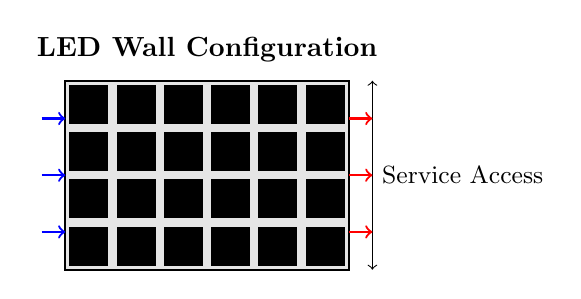
\begin{tikzpicture}[scale=0.6]
    % Draw LED wall cross-section
    \draw[thick, fill=gray!20] (0,0) rectangle (6,4);
    
    % LED modules
    \foreach \x in {0.5,1.5,2.5,3.5,4.5,5.5} {
        \foreach \y in {0.5,1.5,2.5,3.5} {
            \draw[fill=black] (\x-0.4,\y-0.4) rectangle (\x+0.4,\y+0.4);
        }
    }
    
    % Service access
    \draw[<->] (6.5,0) -- (6.5,4);
    \node[right] at (6.5,2) {\small Service Access};
    
    % Cooling arrows
    \foreach \y in {0.8,2,3.2} {
        \draw[->, thick, blue] (-0.5,\y) -- (0,\y);
        \draw[->, thick, red] (6,\y) -- (6.5,\y);
    }
    
    \node[above] at (3,4.2) {\textbf{LED Wall Configuration}};
\end{tikzpicture}
\caption{Cross-section view of LED wall showing modular construction}
\end{figure}

\subsubsection{Option B: Laser Projection Specification}

\textbf{Projector Requirements:}
\begin{itemize}
    \item 3-chip DLP laser projectors
    \item Native 4K resolution (4096×2160) minimum
    \item 20,000-40,000 lumens per projector
    \item RGB laser or laser-phosphor technology
    \item 120 Hz native, 240+ Hz capability
\end{itemize}

\textbf{Remote Light Engine Technology:}
\begin{itemize}
    \item Digital Projection Satellite MLS or equivalent
    \item Light source separation up to 100m via fibre
    \item Noise level <25 dB(A) in cave space
    \item Centralised cooling in equipment room
\end{itemize}

\textbf{Screen Specifications:}
\begin{itemize}
    \item Rigid rear-projection screens for walls
    \item High gain (~1.5) with ambient light rejection
    \item Colour-neutral surface for stereo preservation
    \item Minimal edge gaps with blend overlap zones
\end{itemize}

\subsection{Compute Backend Requirements}

\subsubsection{GPU Cluster Specification}

\begin{table}[h]
\centering
\begin{tabular}{|l|l|}
\hline
\textbf{Component} & \textbf{Specification} \\
\hline
GPU Count & Minimum 32 high-performance GPUs \\
\hline
GPU Model & NVIDIA RTX 6000 Ada or newer \\
\hline
Cluster Architecture & 4 nodes × 8 GPUs or 8 nodes × 4 GPUs \\
\hline
CPU & Dual Xeon or AMD EPYC per node \\
\hline
RAM & 256+ GB per node, 1-2 TB aggregate \\
\hline
Interconnect & NVLink/NVSwitch within nodes \\
 & InfiniBand or 200+ Gbps between nodes \\
\hline
Synchronisation & Hardware genlock/framelock \\
 & Sub-0.1ms sync accuracy \\
\hline
\end{tabular}
\caption{Compute cluster specifications}
\end{table}

\subsubsection{Software Stack Requirements}

\textbf{Visualisation Engines:}
\begin{itemize}
    \item Unreal Engine 5 with nDisplay
    \item Unity 2025 with cluster plugins
    \item NVIDIA Omniverse for RTX rendering
\end{itemize}

\textbf{System Software:}
\begin{itemize}
    \item Linux (Rocky/RedHat/Ubuntu LTS) or Windows
    \item Container support (Docker/Kubernetes)
    \item Cluster management and orchestration
    \item Calibration software (Scalable Display/VIOSO)
\end{itemize}

\subsection{Audio System Requirements}

\subsubsection{Wave Field Synthesis Array}

\begin{itemize}
    \item 128-512 independently driven loudspeakers
    \item Full-range drivers (100 Hz - 20 kHz)
    \item Speaker spacing <30cm for proper synthesis
    \item Two-level array for vertical localisation
    \item Maximum SPL >90 dB at 1m continuous
    \item System peaks of 100+ dB SPL capability
\end{itemize}

\begin{figure}[h]
\centering
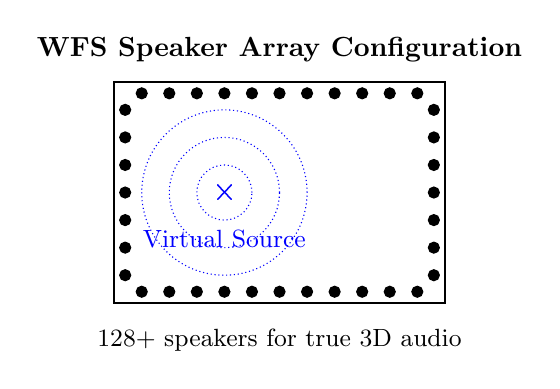
\begin{tikzpicture}[scale=0.7]
    % Draw room outline
    \draw[thick] (0,0) rectangle (6,4);
    
    % Draw speaker arrays
    \foreach \x in {0.5,1,1.5,2,2.5,3,3.5,4,4.5,5,5.5} {
        \draw[fill=black] (\x,0.2) circle (0.1);
        \draw[fill=black] (\x,3.8) circle (0.1);
    }
    \foreach \y in {0.5,1,1.5,2,2.5,3,3.5} {
        \draw[fill=black] (0.2,\y) circle (0.1);
        \draw[fill=black] (5.8,\y) circle (0.1);
    }
    
    % Sound waves
    \draw[blue, densely dotted] (2,2) circle (0.5);
    \draw[blue, densely dotted] (2,2) circle (1);
    \draw[blue, densely dotted] (2,2) circle (1.5);
    
    % Virtual source
    \node[blue] at (2,2) {\textbf{×}};
    \node[blue, below] at (2,1.5) {\small Virtual Source};
    
    % Labels
    \node[above] at (3,4.2) {\textbf{WFS Speaker Array Configuration}};
    \node[below] at (3,-0.3) {\small 128+ speakers for true 3D audio};
\end{tikzpicture}
\caption{Wave Field Synthesis speaker array layout}
\end{figure}

\subsubsection{Processing and Amplification}

\begin{itemize}
    \item Dedicated WFS DSP server/appliance
    \item Support for N sources over M speakers at 60+ FPS
    \item Multichannel amplifiers (8-16 channels per unit)
    \item Network control and monitoring
    \item Low latency (<5ms added delay)
\end{itemize}

\subsection{Tracking and Capture Requirements}

\subsubsection{Optical Motion Tracking}

\begin{table}[h]
\centering
\begin{tabular}{|l|l|}
\hline
\textbf{Parameter} & \textbf{Requirement} \\
\hline
Camera Count & 8-16 high-speed tracking cameras \\
\hline
Camera Speed & $\geq$240 Hz capture rate \\
\hline
Accuracy & $\leq$1mm throughout volume \\
\hline
Latency & <10ms from capture to data \\
\hline
Tracked Objects & 6 users + 2 controllers minimum \\
 & 20 rigid bodies + 10 markers total \\
\hline
Tracking Volume & Full cave interior coverage \\
\hline
Marker Type & Active LED or passive reflective \\
\hline
\end{tabular}
\caption{Motion tracking system requirements}
\end{table}

\subsubsection{Volumetric Capture System}

\textbf{Camera Array:}
\begin{itemize}
    \item 32-64 RGB cameras (4K minimum)
    \item 60-120 fps capture rate
    \item Global shutter with genlock
    \item Hardware synchronisation (<1µs)
\end{itemize}

\textbf{Processing Requirements:}
\begin{itemize}
    \item Dedicated reconstruction server
    \item 8+ GPUs for real-time processing
    \item 30 fps reconstruction target
    \item 1-2 million polygon output
    \item <100ms capture-to-render latency
\end{itemize}

\subsection{Network Infrastructure Requirements}

\subsubsection{Internal Network Fabric}

\begin{itemize}
    \item Non-blocking spine-leaf architecture
    \item 100 Gbps to each compute/storage node
    \item 1+ Tbps aggregate fabric capacity
    \item RDMA support (RoCE v2 or InfiniBand)
    \item PTP time synchronisation
\end{itemize}

\subsubsection{External Connectivity}

\begin{itemize}
    \item Dual 100 GbE uplinks to campus
    \item Connection to JANET network
    \item Secure VPN for remote support
    \item Firewall with appropriate security
\end{itemize}

\subsection{Performance Requirements Summary}

\begin{table}[h]
\centering
\begin{tabular}{|l|l|}
\hline
\textbf{Metric} & \textbf{Target} \\
\hline
End-to-end latency & <20ms motion-to-photon \\
\hline
Tracking jitter & <1mm position variance \\
\hline
Visual acuity & $\geq$1 arcminute/pixel \\
\hline
Brightness uniformity & >90\% across surfaces \\
\hline
Colour accuracy & $\Delta$E < 2 \\
\hline
Audio localisation & <1° error anywhere \\
\hline
System uptime & >95\% availability \\
\hline
\end{tabular}
\caption{Key performance requirements}
\end{table}